
\section{The system studied}
Since the strong decay $\phi \rightarrow K^0 \overline{K}^0$ conserves angular momentum and CP eigenvalues, the two kaons form an antisymmetric state which can be written as %$J^{PC}(\phi) = 1^{--}$, $J^{PC}(K^0, \bar{K^0}) = 0^{--}$,$C = (-1)^\ell$, $P    =(-1)^\ell$
\begin{equation}
|\phi\rangle \rightarrow \frac{1}{\sqrt{2}}\left(\left|K^0 \overline{K}^0\right\rangle - \left| \overline{K}^0K^0\right\rangle\right) = \frac{\mathcal{N}}{\sqrt{2}} \left(\left|K_SK_L\right\rangle - \left|K_LK_S\right\rangle\right)
\end{equation}
where $\mathcal{N} = \frac{1+|\epsilon|^2}{1-\epsilon^2}$ and $\left|K_S\right\rangle = \frac{1}{\sqrt{1+|\epsilon|^2}}\left(\left|K_+\right\rangle + \epsilon \left| K_-\right\rangle\right)$ as well as $\left|K_L\right\rangle = \frac{1}{\sqrt{1+|\epsilon|^2}}\left(\left|K_+\right\rangle + \epsilon \left| K_-\right\rangle\right)$. The states $|K^0\rangle$ and $|\overline{K}^0\rangle$ are flavor eigenstates, $\left|K_S\right\rangle$ and $\left|K_L\right\rangle$ are mass eigenstates in which the kaons propagate, and $\left|K_+\right\rangle$ and $\left|K_-\right\rangle$ are CP eigenstates. Because the mass eigenstates and the CP eigenstates are not equivalent, CP is violated, i.e. both $K_S$ and $K_L$ can decay into two charged pions with $\mathcal{B}(K_S \rightarrow \pi^+ \pi^-) = (69.20\pm0.05)\%$ and $\mathcal{B}(K_L \rightarrow \pi^+ \pi^-) = (1.967\pm0.010)\cdot 10^{-3}$ respectively \cite{Agashe:2014kda}.  These two decays lead to an interference term in the decay intensity

\begin{equation}
I(t_1,t_2) \propto  e^{-\Gamma_L t_1 - \Gamma_S t_2} +e^{-\Gamma_S t_1 - \Gamma_L t_2}- 2 e^{-\frac{1}{2}\left(\Gamma_S + \Gamma_L\right)\left(t_1+t_2\right)}\cos\left(\Delta m \left(t_1-t_2\right)\right) \label{EQ:DI1}
\end{equation}
where $t_{1,2}$ are the decay times of the two kaons, $\Gamma_{S,L}$ are the decay widths of $K_S$ and $K_L$, and $\Delta m = \left|m_{K_L} - m_{K_S}\right|$ is the mass difference between them. The effects of a non-unitary time evolution due to CPT violation can be parameterized by introducing a decoherence term $\zeta_{SL}$\cite{Balwierz-Pytko:2013xsa}.

\begin{equation}
I(t_1,t_2) \propto  e^{-\Gamma_L t_1 - \Gamma_S t_2} +e^{-\Gamma_S t_1 - \Gamma_L t_2}- 2(1-\zeta_{SL}) e^{-\frac{1}{2}\left(\Gamma_S + \Gamma_L\right)\left(t_1+t_2\right)}\cos\left(\Delta m \left(t_1-t_2\right)\right). \label{EQ:DI2}
\end{equation}

Though there are many different models that describe CPT violation, this study will only consider this one. 

If $\zeta_{SL}$ is non-zero, this manifests itself in an excess of decays with small decay time differences $\Delta t = |t_1 - t_2|$ as shown in figure \ref{FIG:Excess}.
\newpage
\hspace*{3.2cm}$I(\Delta t)$[a.u.]
\vspace*{-.3cm}
\begin{center}
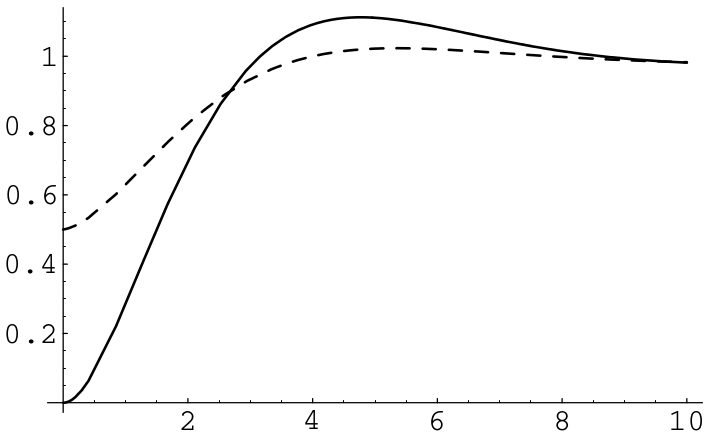
\includegraphics[width = .5\textwidth]{figs/Excess.png}
\end{center}
\vspace*{-.4cm}\hspace*{12cm}$\Delta t/\tau_S$
\captionof{figure}{Decay intensity $I(\Delta t)$ of $\phi\rightarrow \pi^+\pi^-\pi^+\pi^-$. The solid line is for $\zeta_{SL}=0$ and the dashed line for $\zeta_{SL}\neq 0$. \cite{Bernabeu:2006st} \label{FIG:Excess}}

\vspace*{.5cm}

The currently best 95\% C.L. limit on this parameter is set by KLOE with $\zeta_{SL} = 0.098$ \cite{Ambrosino2006315}.


\subsection{$\phi$ Production channels}

At LHCb, two $\phi$ production channels can be taken into consideration to do this study. One uses prompt $\phi$ coming directly from the primary vertex and the other uses $\phi$ from the decay $D_s^\pm \rightarrow \phi \pi^\pm$. Both production channels are illustrated in figure \ref{FIG:tracks}.
\vspace*{.5cm}
\begin{center}
\begin{minipage}{.49\textwidth}\centering
\begin{fmffile}{incl}
		\setlength{\unitlength}{.5mm}
		\fmfframe(0,0)(10,10){
		\begin{fmfgraph*}(75,65)
			\fmfleft{l1}
			\fmfright{r1,r2,r3,r4}
			\fmflabel{$\pi^+$}{r1}
			\fmflabel{$\pi^-$}{r2}					
			\fmflabel{$\pi^+$}{r3}
			\fmflabel{$\pi^-$}{r4}
			\fmf{plain}{r1,x1,r2}
			\fmf{plain}{r3,x2,r4}
			\fmf{dashes,label=$K^0$}{x1,y1}
			\fmf{dashes,label=$\overline{K}^0$}{y1,x2}
			\fmf{dashes,label=$\phi$}{l1,y1}
			\fmfforce{(.2w,.5h)}{y1}
		\end{fmfgraph*}}
\end{fmffile}
\end{minipage}
\begin{minipage}{.49\textwidth}\centering
\begin{fmffile}{Ds}
		\setlength{\unitlength}{.5mm}
		\fmfframe(0,0)(10,10){
		\begin{fmfgraph*}(75,65)
			\fmfleft{l1}
			\fmfright{r1,r2,r3,r4,r5}
			\fmflabel{$\pi^+$}{r1}
			\fmflabel{$\pi^-$}{r2}					
			\fmflabel{$\pi^+$}{r3}
			\fmflabel{$\pi^-$}{r4}
			\fmf{plain}{r1,x1,r2}
			\fmf{plain}{r3,x2,r4}
			\fmf{dashes,label=$K^0$}{x1,y1}
			\fmf{dashes,label=$\overline{K}^0$}{y1,x2}
			\fmf{dashes,label=$\phi$}{z1,y1}
			\fmf{plain}{l1,z1}
			\fmf{plain}{z1,r5}
			\fmflabel{$D_S^\pm$}{l1}
			\fmflabel{$\pi^\pm$}{r5}
		\end{fmfgraph*}}
\end{fmffile}
\end{minipage}
\captionof{figure}{Topology of prompt $\phi$ production (left) and $D_s^\pm \rightarrow \phi \pi^\pm$ (right) and the decay $\phi\rightarrow K^0 \overline{K}^0\rightarrow \pi^+\pi^-\pi^+\pi^-$. Solid lines indicate charged particles with tracks, dashed lines indicate neutral particles.} \label{FIG:tracks}
\end{center}

Including a cut on LHCb's geometric acceptance, the production cross sections for \SI{14}{TeV} as extrapolated from the \SI{7}{TeV} cross sections are for prompt $\phi$ \SI{3516}{\micro b} \cite{Aaij:2011uk} and for $D_s^\pm$ \SI{388}{\micro b} \cite{LHCb-CONF-2010-013}. Additionally, the branching fraction $\mathcal{B}(D_s^\pm \rightarrow \phi \pi^\pm) = (4.5 \pm 0.4)\%$ has to be taken into account for the production rate of $\phi$ in the $D_s^\pm$ channel. Both approaches are considered because the production rate of prompt $\phi$ is considerably higher than that of $\phi$ from $D_s^\pm$ decays, but $D_s^\pm \rightarrow \phi\pi^\pm$ might offer a better handle on background rejection because of the displaced $D_s^\pm$ vertex and a constraint on the $D_s^\pm$ mass.

\subsection{Background processes}

If one considers the excess of $\phi \rightarrow K^0 \overline{K}^0 \rightarrow \pi^+ \pi^- \pi^+ \pi^-$ for small $\Delta t$ due to CPT violation as signal, there are three main sources of background. One is the decay mode $\phi \rightarrow K_L K_S \rightarrow \pi^+\pi^-\pi^+\pi^-$ resulting from CP violation which from here one is going to be referred to as Standard Model (SM) background. Its decay intensity is plotted as the solid line in figure \ref{FIG:Excess}. The second background is so called regeneration background which results from the interaction of $K_L$ with matter and causes a transformation $K_L \rightarrow K_S$. The third background is combinatoric background of prompt kaons and pions.

\subsection{Track types}

In LHCb, different track types are defined depending on the sub-detectors in which the hits used to reconstruct the track are located. A schematic overview of the track types is given in figure \ref{FIG:tracktype}. For this study, we will consider only long tracks which are reconstructed with hits in the Velo (Vertex locator) and the other components of the tracking system, and downstream tracks which do not have hits in the Velo. Depending on its decay time a kaon can decay inside or outside the Velo and thus be reconstructed using two long pion tracks (LL) or two downstream pion tracks (DD). Kaons with long decay times are reconstructed using downstream tracks and kaons with short decay times are reconstructed using long tracks.


\begin{center}
    \def\svgwidth{.9\textwidth}
    \input{image.pdf_tex}
\captionof{figure}{Track types in LHCb: Upstream tracks are in the Velo and TT, downstream tracks in both outer trackers, and long tracks in all trackers. \cite{tracktypes}}\label{FIG:tracktype}
\end{center}
